\chapter{Poset}
\label{ch-poset}

A {\bf partially order set or poset}
$(P, \pord )$
consists of a set $P$ for  which a relation $\pord\;: P\times P\rarrow \{True, False\} $ is defined. For all $a,b,c\in P$, the  relation must
satisfy:

\begin{enumerate}
\item
{\bf reflexivity:}
$a\pord  a$

\item
{\bf symmetry:}
if $a\pord  b$ and $b\pord  a$ then $a=b$.

\item{\bf transitivity:}
if $a\pord  b$ and $b\pord  c$ then $a\pord  c$.

Given a general poset $(P, \pord)$ with two elements $a, b\in P$,
if we can find a path  $a\pord x_1 \pord x_2\pord\ldots\pord b$,
or a path connecting $a$ and $b$  in the other direction,  then we say $a$ and $b$ are {\bf comparable}.
Actually, the statement that \qt{there is
a path $a\pord x_1 \pord x_2\pord\ldots\pord b$}
is  equivalent to saying that
$a\pord b$, and  the statement that \qt{there is a path in the
opposite direction},  is equivalent to
saying that $b\pord a$. Hence,
$a, b\in P$ are comparable iff $a\pord b$ or $b\pord a$;
and they are {\bf non-comparable}
iff neither is true.
General posets can have
non-comparable elements.
A {\bf total order} is a poset
in which all elements are comparable.

\end{enumerate}

A {\bf strict poset} $(P, \spord )$
consists of a set $P$ on which a relation $\spord\;: P\times P\rarrow \{True, False\} $ is defined. For all $a,b,c\in P$, the  relation must
satisfy:

\begin{enumerate}
\item
{\bf anti-reflexivity:}
No element $a\in P$ satisfies $a\spord  a$

\item
{\bf anti-symmetry:}
if $a\spord b$ then
not  $b\spord a$

\item{\bf transitivity:}
if $a\spord  b$ and $b\spord  c$ then $a\spord  c$

\end{enumerate}
\begin{figure}[h!]
$$
\bcen
\xymatrix@R=1pc{
&5\ar[dl]\ar[dr]
\\
3\ar[dr]
&&4\ar[dl]
\\
&2\ar[d]
\\
&1
}
\ecen
\quad
\ol{M}=
\begin{pmatrix}
1&1&1&1&1
\\
0&1&1&1&1
\\
0&0&1&0&1
\\
0&0&0&1&1
\\
0&0&0&0&1
\end{pmatrix},\quad
M=
\begin{pmatrix}
0&1&1&1&1
\\
0&0&1&1&1
\\
0&0&0&0&1
\\
0&0&0&0&1
\\
0&0&0&0&0
\end{pmatrix}
$$
\caption{HD and two logic matrices that it represents. The logic matrix $\ol{M}$ is for a  poset, and the logic matrix ${M}$ is for the corresponding strict
poset. Note that $M$ and $\ol{M}$ have identical nondiagonal entries.
Along the diagonal,
$\ol{M}$
has only ones and $M$ has only zeros.
We don't do this, but
the links in a HD are often depicted without arrowheads. In that case, the arrows are implicit rather than explicit and can be assumed  to be all pointing downwards.}
\label{fig-logic-matrices}
\end{figure}


A {\bf logic matrix}
for a poset $(P,  \pord )$ (resp., strict poset $(P, \spord)$) is a matrix $\ol{M}$ (resp., $M$) such that

\beq
\ol{M}_{ab} =\indi(a \pord  b) \quad \text{ ( resp., $M_{ab} =\indi(a \spord  b)$)}
\eeq
for all $a, b\in P$.
Fig.\ref{fig-logic-matrices}
gives an example of a
logic matrix for a poset and its corresponding strict poset.

Apart from a logic matrix, the following 2 types of diagrams can be used to represent a poset:

\begin{enumerate}

\item A {\bf DAG} is a directed acyclic graph. It represents a bnet.

In a DAG, we say an {\bf arrow
$\rvx\rarrow \rvy$ is transitive}  if there is a node $\rvm$ \qt{in between} $\rvx$ and $\rvy$ ; i.e.,  if there is
a node $\rvm$ and arrows $\rvx\rarrow \rvm$, $\rvm\rarrow \rvy$.
A DAG can be used to represent a
poset but not all DAGs represent a poset. That's because a DAG can contain some
but not all of the transitive arrows whereas a poset, if   represented by a DAG,
would include ALL transitive arrows
and even self-interaction loops
(which
violate acyclicity)
in the poset case.

\item A {\bf Hasse diagram (HD)} is a minimal representation of a poset.
By this we mean that
it contains an arrow $\rva\larrow \rvb$ iff $\rva \pord \rvb$ and there is no
$\rvx$ such that $\rva\pord \rvx\pord \rvb$.
Hence, a HD is a DAG
without any transitive arrows (indirect relations).
Also, a HD has no self-interaction loops
in the poset case.
See Fig.\ref{fig-logic-matrices} for an example
of a HD.
\end{enumerate}

A {\bf lattice} is a poset $(P, \pord)$ equipped with two binary operations $\A\;: P\times P\rarrow P$ and $\V\;: P\times P\rarrow P$, such that, for every pair $a, b\in P$,

\begin{enumerate}
\item there exists a unique {\bf supremum (sup)} (a.k.a join)
denoted by $a\A b$.
By a supremum, we mean an element $sup\in P$
which satisfies

\beq
a\pord sup, \quad b\pord sup
\eeq
and is the largest element
of $P$ to do so.


\item there is  a unique
{\bf infimum (inf)}, (a.k.a. {meet}) denoted by $a\V b$.

By an infimum, we mean an element $inf\in P$
which satisfies

\beq
inf \pord a, \quad inf\pord b
\eeq
and is the smallest element
of $P$ to do so.
\end{enumerate}





\begin{claim} \label{cl-relation-pord-and-or}
The following are
equivalent:

\begin{enumerate}[(a)]

\item
$a\pord b$

\item
$a\A b =b$


\item
$a \V b =a$
\end{enumerate}
Hence, when the pair $a,b\in P$ is comparable,  its sup (resp., inf) is simply the element of the pair that is further upstream (resp., further downstream).
\end{claim}
\proof

This claim follows
from the definitions of sup and inf.
\qed


 Fig.\ref{fig-Hasse-sup-inf} shows the HD
for the  lattice $D_{12}=$ divisors of 12.
In this lattice, each node is a common factor (the largest possible one not equal to the parents)
of its parents. In other words, each node is the greatest common divisor (gcd) of its parents. If $d$ divides $x$, one denotes this by $d|x$
For this HD,
$a\pord b \iff a|b$.

The power set $\calp(S)$ of a set $S$ is the set of all
subsets of $S$, including $S$  and the
empty set.
 Fig.\ref{fig-pow-set-123} shows the HD of the lattice $\calp(\{1,2,3\})$.
In this figure, each
node is a subset (the largest possible one not equal to the parents) of its parents. In other words,
every node is the intersection of its parents.
Furthermore, $A\A B= A\cap B$ and
$A\V B= A\cup B$
for $A, B\subset \{1,2,3\}$.

\begin{figure}[h!]
\centering
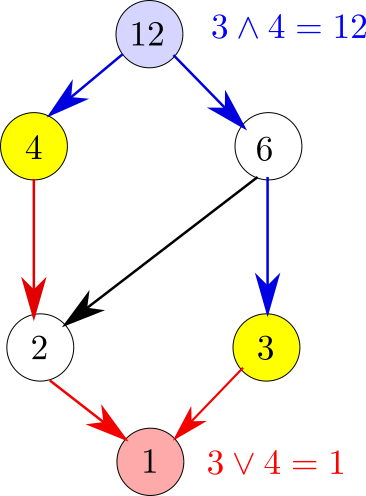
\includegraphics[width=1.5in]
{poset/join-meet.png}
\caption{HD
for the lattice $D_{12}$=divisors of 12. 3 and 4 are not comparable but 4 and  1 are. $3\A4=12$ and $3\V 4=1$. Also
$4\A 1 =4$ and $4\V 1=1$. Hence, $\V$ and $\A$ are defined for all pairs, regardless of whether the pair is comparable or not.
When a pair $a,b\in P$ is comparable,  its sup (resp., inf) is simply the element
of the pair that is further upstream (resp., further downstream).}
\label{fig-Hasse-sup-inf}
\end{figure}

\begin{figure}
$$
\xymatrix{
&\{1,2,3\}
\ar[dl]
\ar[d]\ar[dr]
&
\\
\{1,2\}
\ar[d]
\ar[dr]
&\{1,3\}
\ar[dl]
\ar[dr]
&\{2,3\}
\ar[d]
\ar[dl]
\\
\{1\}
\ar[dr]
&\{2\}
\ar[d]
&\{3\}
\ar[dl]
\\
&
\varnothing
}
$$
\caption{HD for the lattice $\calp(\{1,2,3\})$}
\label{fig-pow-set-123}
\end{figure}

It's also possible to define a lattice backwards.
\begin{itemize}
\item (our approach so far) assume a lattice is a poset with a partial order
relation $\pord$ and then define the binary operations $\A, \V$
in terms of $\pord$
\item (algebraic approach)
assume the binary operations $\A, \V$
satisfy a bunch of axioms for AND and OR operators (Boolean algebra), and then
define the relation
$\pord$ in terms of
$\A$ and $\V$
\end{itemize}
We won't say anymore about the algebraic approach. You can look
it up if it interests you.

In the HD of Fig.\ref{fig-pow-set-123}, let

$\Omega =\{1,2,3\}=$ probability outcome space

$\omega\in \Omega$. We will represent
all elements of $\Omega$
by lower case Greek letters.

$x\in \bool$. We will represent all Boolean variables by lower case
Latin letters.
As we shall see,
it's important to make this
distinction in the
notation between elements $\omega$ of the outcome
space and elements $x$ of $\bool$. Not making the distinction can lead to a lot
of confusion and contradictions.


$S\subset \Omega$. We will represent all subsets of $\Omega$ by capital Latin letters.

$\indi_{S}(\omega)= \indi(\omega\in S)$
for $S\subset \Omega$. Note that the function $\indi_{S}$ maps  $\Omega\rarrow \bool$,
so, by definition, it is a random variable
with $val(\indi_S)=\bool$.
So $\indi_S$ is a
random variable
and $\indi_S(\omega)$
is a Boolean variable.


\beq
P(\indi_S= x)=P(\{\omega\in \Omega : \indi_S(\omega)=x\})=P(S)\delta_1^x + P(S^c)\delta_0^x
\eeq

In the HD of Fig.\ref{fig-pow-set-123}, we can replace
the set $S$ labeling each node by its indicator function $\indi_S$. Hence, if a node has parents $\indi_{A}$ and $\indi_B$, then the node is

\beq
\indi_{A\cap B}= \indi_A \indi_B =
\indi_A \A \indi_B
\eeq
This is why
the lattice
represented by the HD of Fig.\ref{fig-pow-set-123} is called both
the lattice for the power set of 3 elements,
and the {\bf Boolean lattice} for 3 Boolean variables. Note that a Boolean lattice is a special
kind of lattice
that has extra properties than a generic lattice
does not have.

